\section{Prácticos realizados}
\subsection{BCD $\rightarrow$ Exceso-3}
\textbf{Consigna:}
Diseñar y armar un conversor de código BCD a XS3 (exceso 3). Realizar: \begin{enumerate} \item Tabla de verdad \item Obtener las funciones lógicas de calidas con circuitos combinacionales. \item Minimizar el circuito y verificar su funcionamiento en el MiniLab. \item Armar el circuito y verificar su funcionamiento en el simular ''falstad.com'' \end{enumerate}

\subsection{Comparador binario}

El siguiente circuito es un comparador binario de dos números $A$ y $B$ de dos bits cada uno. Las salidas ($S0$, $S1$ y $S2$) representan la salida del comparador y cuando $S0 = 1$ cuando $A>B$ y $S2 = 1$ para $A = B$, en caso de no darse la condición, la salida permanece en cero.

\begin{center}
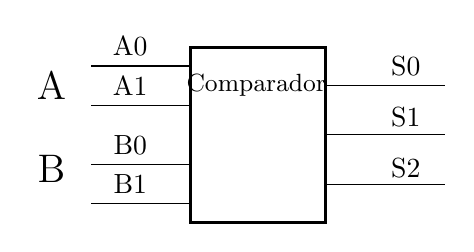
\begin{tikzpicture}
	\node[shape=rectangle, draw, line width=1pt, inner sep=0, minimum width=1.715cm, minimum height=2.215cm] at (5.125, 3.125){};
	\draw (4.25, 4) -- (3, 4);
	\draw (4.25, 3.5) -- (3, 3.5);
	\draw (4.25, 2.25) -- (3, 2.25);
	\draw (4.25, 2.75) -- (3, 2.75);
	\draw (6, 2.5) -- (7.5, 2.5);
	\draw (6, 3.75) -- (7.5, 3.75);
	\draw (6, 3.125) -- (7.5, 3.125);
    \node at (3.5, 4.25) {A0};
    \node at (3.5, 3.75) {A1};
    \node at (3.5, 3) {B0};
    \node at (3.5, 2.5) {B1};
    \node at (7, 4) {S0}; 
    \node at (7, 3.35) {S1};
    \node at (7, 2.7) {S2};
    \node at (5.1 , 3.75) {\small Comparador};
    \node at (2.5, 3.75) {\Large A};
    \node at (2.5, 2.7) {\Large B};
\end{tikzpicture} \end{center}

Se pide:
\begin{enumerate} \item Tabla de verdad. \item Obtener las funciones lógicas de salidas con circuitos combinacionales. \item Circuito mínimo usando mapa de Karnaugh. \item Circuito mínimo usando teoremas y postulados de álgebra de Boole. \item Armado de circuito y verificado en MiniLab. \item Armado de circuito y verificado con simulador ''falstad.com'' \end{enumerate}
